\chapter{Algoritmo}\label{cap.algoritmo}

\hspace{1 cm} En este cap\'itulo se describe el modo por el cual, con la infraestructura que se tiene, se llega a una soluci\'on para lo planteado en los objetivos. 

\hspace{1 cm} Este algoritmo tiene que permitir al drone despegar de forma controlada, realizar una navegaci\'on autonoma para encontrar una baliza sobre la que aterrizar. La organizaci\'on de este cap\'itulo tiene primero una secci\'on de diseño, en el que se explica el funcionamiento del programa. Tras esto una secci\'on de percepci\'on para explicar los datos que se obtienen a trav\'es de los sensores, y para finalizar una secci\'on de control, para explicar los distintos movimientos del drone y de que dependen estos.

\section{Diseño}
\label{sec.Design}

\hspace{1 cm} El diseño de este algoritmo consta de un comportamiento reactivo de iteraciones continuas. Es un proceso basado en adquisici\'on-procesado-env\'io de datos. La adquisici\'on de los datos se realizan mediante los sensores del drone. Estos datos ser\'an transmitidos al dispositivo para que lo procese y tras estos se enviar\'an las instrucciones al drone para que este las ejecute. El sensor utilizado en este proyecto ha sido la c\'amara, y los movimientos del drone depender\'an de lo que esta capte en cada momento. 

\hspace{1 cm} Por otro lado, la parte es un aut\'omata finito de estados, el cual comienza en un estado inicial (despegue), y en funci\'on de lo que recibe a la entrada (imagen del sensor), realizar\'a el procesamiento necesario para producir la informaci\'on que enviar al drone, y en ocasiones le llevar\'a a pasar de un estado a otro. Destacar que este aut\'omata est\'a compuesto por 6 estados: despegue, busqueda, posible baliza, centr\'andose en la baliza, aterrizando y aterrizado. A excepci\'on del primero, los dem\'as estados depender\'an de lo que detecte el drone en cada momento. El primer estado esta controlado por tiempo, pues son 10 segundos al iniciarse en los que el drone inicia el vuelo sobre una baliza y trata de estar centrado sobre esta, para as\'i tener un despegue controlado y evitar que el drone se mueva en caso de tener alguna deriva o haya factores externos que produzcan esto. Una vez transcurridos los 10 segundos se pasar\'a al estado de b\'usqueda e ira pasando por los distintos estados hasta su aterrizaje. 

\begin{figure}[H]
	\centering
		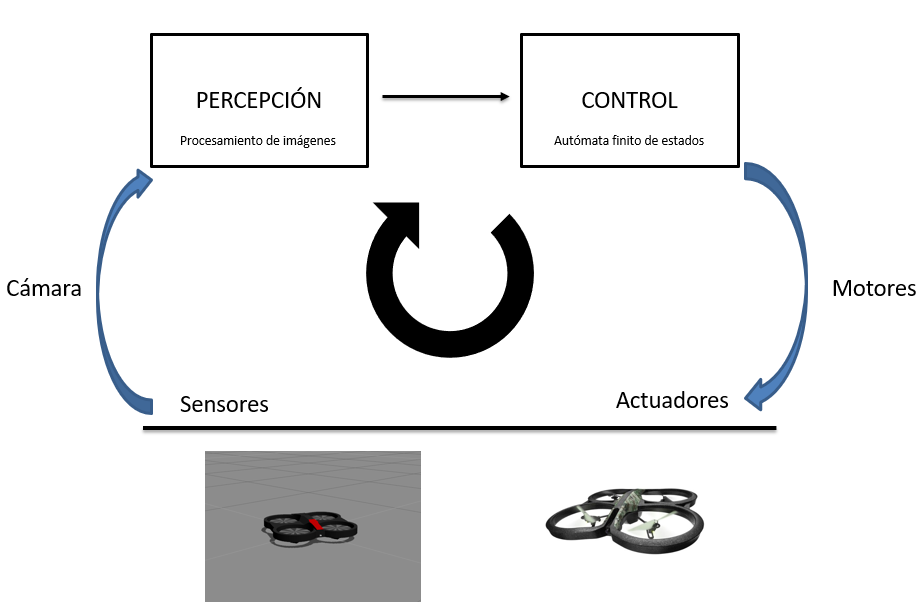
\includegraphics[width=0.75\textwidth]{imgs/esquema2.png}
	\label{fig:esquema_d}
\end{figure}

\hspace{1 cm} El lugar de aterrizaje del drone es una baliza previamente definida. Esta baliza es un cuadrado que en su interior tiene cuatro cuadrados, dos naranjas, y dos azules o verdes, dependiendo si se trabaja con el drone real o con el simulador. Esta baliza se ha elegido para que sea dif\'icil confundirla con otro objeto, pues de ser una baliza simple se podr\'ian confundir los colores. De esta forma lo que buscaremos ser\'a la cruceta que forman estos cuatro cuadrados y el punto central de \'esta. Por lo tanto, en lugar de un objeto en si lo que se busca es un objeto que tenga determinadas caracter\'isticas y patrones, algo que se puede detectar a diferentes alturas, distintas condiciones y situaciones.

\begin{figure}[H]
	\centering
		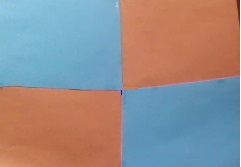
\includegraphics[width=0.3\textwidth]{imgs/baliza.jpg}
         \caption{Baliza utilizada para el drone real.}
	\label{fig:esquema_d}
\end{figure}


\hspace{1 cm} Por \'ultimo, para el control del drone con nuestro algoritmo se ha utilizado la herramienta follow\_turtlebot de JdeRobot Academy, explicada en \ref{sec.JdeRobotAcademy} . \'Esta aplicaci\'on tiene un interfaz gr\'afico de usuario (GUI) que permite controlar el drone y ver los datos de los distintos sensores, as\'i como la imagen que obtiene la c\'amara. Por otro lado cuenta con las interfaces ICE que permite la comunicaci\'on con el servidor, pudiendo as\'i recibir datos de sensores y motores, y enviar las instrucciones de velocidad necesarias en cada momento. La imagen de la aplicaci\'on se encuentra en la figura \ref{fig:FollowTurtlebot}


\section{Percepci\'on}

\hspace{1 cm} En \'esta secci\'on se va a tratar la obtenci\'on de la imagen de la c\'amara y el procesamiento que se realiza sobre \'esta. Gracias a lo que el drone ve en todo momento, sabe el punto del proceso en el que se encuentra y la informaci\'on que debe enviar. En primer lugar, se obtiene una imagen de entrada, esta imagen es procesada con filtros de color y operadores morfol\'ogicos, obteniendo una imagen de salida. A partir de los datos de \'esta imagen, se detecta si hay objetos de inter\'es o no, y por tanto se env\'ia unas instrucciones u otras al drone. 


\subsection{Pre-procesado}

\hspace{1 cm} Una vez tenemos la imagen de entrada, hay que detectar la informaci\'on de interes que nos aporta. 
 
\hspace{1 cm} En primer lugar, la imagen que est\'a en RGB se transforma a HSV, para que sea mas facil su interpretaci\'on, ya que en lugar de trabajar en funci\'on de tres colores (rojo, verde y azul), se trabaja en funci\'on de tres par\'ametros (tono, saturaci\'on y valor). De \'esta forma, se depende menos de la luz que haya en cada momento y en cada lugar. En el filtro, a cada uno de los parametros se le asigna un rango de valores entre 0 y 255. La herramienta colorTuner permite, a partir de una imagen de entrada, dar valores a estos parametros, viendo que objetos cumplen estos requisitos y dejandolos en primer plano, y cuales no, dejando estas zonas en negro como p\'ixeles de fondo. Una vez se obtienen estos valores se añaden al filtro, obteniendo a la salida una imagen que solo muestra los objetos de los colores de inter\'es, dejando el fondo negro. 

\hspace{1 cm} El siguiente c\'odigo es un ejemplo de como, a partir de una imagen de entrada en RGB, se transforma a HSV y se filtran los objetos de color naranja. 

\begin{lstlisting}[backgroundcolor=\color{yellow}]
hsv = cv2.cvtColor(input_image, cv2.COLOR_BGR2HSV)
lower_orange = np.array([100,100,80], dtype=np.uint8)
upper_orange = np.array([150, 255,255], dtype=np.uint8)
maskOrange = cv2.inRange(hsv, lower_orange, upper_orange)
maskRGBOrange = cv2.bitwise_and(input_image,input_image, mask= maskOrange)
\end{lstlisting}


\hspace{1 cm} En caso de trabajar sobre simulador, con esto se obtiene a la salida una imagen bastante parecida a la deseada, debido a la pureza e los colores. Sin embargo, al trabajar sobre im\'agenes reales, la imagen de salida de este filtro a\'un tiene ruido y objetos de inter\'es imperfectos. Para arreglar esto se utilizan los operadores morfol\'ogicos, que eliminan estas imperfecciones. Una breve explicaci\'on de los utilizados es la siguiente: 

\begin{itemize}
	\item \textbf{Erosi\'on:} Dada una imagen y un elemento estructural, la erosi\'on es el conjunto de los elementos \textit{x} para los cuales el elemento estructural trasladado por \textit{x} est\'a contenido en la imagen. 
	\newline\hspace{1 cm} Aplicaci\'on: Cuando un p\'ixel que parece pasar el filtro, pero los elementos de su alrededor(en concordancia con el elemento estructurante) no lo pasan, este pasa a ser parte del fondo. 
	\item \textbf{Dilataci\'on:} Transformaci\'on dual a la erosi\'on. El resultado de esta es el conjunto de elementos tal que al menos alg\'un elemento del conjunto estructurante esta contenido en \textit{x}, cuando el elemento estructurante se desplaza sobre \textit{x}
	\newline\hspace{1 cm} Aplicaci\'on: p\'ixeles que parecen de fondo, pasan a ser de la figura si est\'an cerca de p\'ixeles que pasan el filtro.
	\item \textbf{Cierre:} Se trata de realizar una dilataci\'on en la imagen seguida de una erosi\'on.
	\item \textbf{Apertura:} Se trata de realizar la erosi\'on en una imagen seguido de la dilataci\'on.
\end{itemize}


\hspace{1 cm} De esta forma, al obtener una imagen sin apenas ruido, evitando as\'i que objetos de no inter\'es los detecte como tal y que los objetos de interes los trate como p\'ixeles de fondo. Una im\'agen en la que se observa la realizaci\'on de un filtro de color y el uso de operadores morfol\'ogicos es la siguiente:

\begin{figure}[ht]
	\centering
		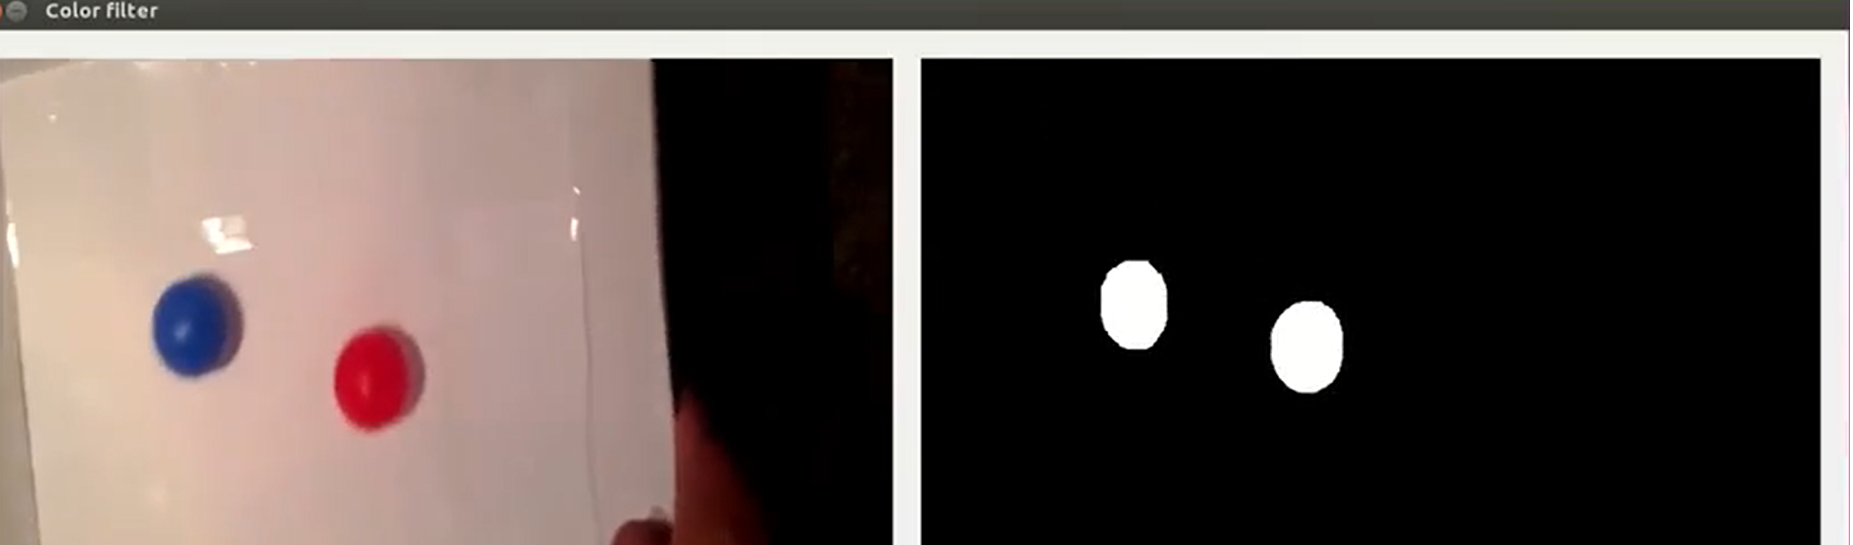
\includegraphics[width=0.8\textwidth]{imgs/colorfilter.eps}
	\label{fig:E_Imagen_baliza}
\end{figure}


\hspace{1 cm} El siguiente fragmento de c\'odigo, muestra como se define la matriz a partir de la cual se realizar\'an las operaciones oportunas, y despues se realizan la erosi\'on y la dilataci\'on.
\begin{lstlisting}[backgroundcolor=\color{yellow}]
kernel = np.ones((3,3),np.uint8)
maskRGBOrange = cv2.erode(maskRGBOrange,kernel,iterations = 4)
maskRGBOrange = cv2.dilate(maskRGBOrange,kernel,iterations = 3)
\end{lstlisting}


\subsection{Detecci\'on de la baliza}
\hspace{1 cm} Una vez se obtienen los colores de los objetos de inter\'es, hay que buscar el objeto deseado. Para \'esto hay que buscar el punto de intersecci\'on entre los cuatro cuadrados de la baliza. Para ello, los pasos a realizar son los siguientes:

\begin{enumerate}
	\item Para la imagen de entrada se hacen dos filtros de color, uno por cada color de la baliza.
	\item De cada imagen se obtienen el n\'umero de objetos, las \'areas y los contornos. En cada objeto se obtiene el valor de su \'area, en caso de ser menor de un valor determinado este se descarta. En caso de tener ese area o mayor, se crea una imagen negra, se pintan los contornos del objeto sobre esta con un valor RGB(0,1,0) y se dilatan. De esta forma, tendremos tantas im\'agenes como objetos. 
	\item Se suman las im\'agenes obtenidas, por lo tanto, sobre una imagen negra final se pintaran los contornos dilatados de todos los objetos. Cada contorno se pintara con un valor RGB(0,1,0), por lo tanto en el caso de que varios objetos coincidan sumar\'an sus valores. Con esto conseguiremos que el punto donde interseccionen cuatro objetos tenga un valor (0,4,0), y por tanto \'este ser\'a el centro de la cruceta.
	
	El siguiente fragmento de c\'odigo muestra la creaci\'on de una imagen por objeto, la dilataci\'on de los contornos y la suma final de las im\'agenes:

\begin{lstlisting}[backgroundcolor=\color{yellow}]
f = []
i=0
imgray2 = cv2.cvtColor(maskRGBOrange,cv2.COLOR_BGR2GRAY)
ret,thresh = cv2.threshold(imgray2,255,255,255)
_,contours, hierarchy = cv2.findContours(thresh,cv2.RETR_TREE,
                                          cv2.CHAIN_APPROX_SIMPLE)
\'areas = [cv2.contour\'area(c) for c in contours]
for extension in \'areas:
    if extension > 100:
    img = np.zeros((y_img*2,x_img*2,3), np.uint8)
        actual = contours[i]
        approx = cv2.approxPolyDP(actual,0.05*cv2.arcLength(actual,True),
                                                                       True)
        cv2.drawContours(img,[actual],0,(0,30,0),12)
        f.append(img)
        i=i+1
			
kernel = np.ones((3,3),np.uint8)
if(len(f)>0):
    f[0] = cv2.dilate(f[0],kernel,iterations = 4)
    show_image2=f[0]
    for k in range(len(f)-1):
        f[k+1] = cv2.dilate(f[k+1],kernel,iterations = 4)
        show_image2=show_image2+f[k+1]
		
\end{lstlisting}


	\item A partir de la imagen final, se pasar\'a un filtro RGB que filtre los valores mayores a RGB(0,3,0), por lo tanto el \'unico valor que no se eliminar\'a sera el del centro de la cruceta.

	\item Sobre la imagen obtenida, utilizando la funci\'on drawcontours, obtenemos la situaci\'on de estos y p\'ixeles, teniendo as\'i la situaci\'on de la cruceta, y con estos valores se puede marcar el centro de la baliza sobre la imagen real. En caso de haber filtrado la intersecci\'on de dos objetos en lugar de cuatro en el apartado anterior, se podr\'ian marcar tambi\'en posibles objetos de inter\'es, como puede ser la baliza completa. 

En el siguiente fragmento de c\'odigo se muestra, como a partir de la imagen de la suma de objetos, se calcula la posici\'on de la cruceta y se marcan sobre la imagen. En \'este caso, para que se obtuviera una imagen mas clara, a los bordes de los objetos se les da un valor de 30, por lo tanto la intersecci\'on de 3 objetos tendr\'a un valor RGB(0,90,0) y de 4 objetos un valor RGB(0,120,0).

\begin{lstlisting}[backgroundcolor=\color{yellow}]
lower_green = np.array([0,80,0], dtype=np.uint8) 
upper_green = np.array([0, 140,0], dtype=np.uint8) 
maskSHI = cv2.inRange(show_image2, lower_green, upper_green)
show_image2 = cv2.bitwise_and(show_image2,show_image2, mask= maskSHI)

compare_image = np.zeros((y_img*2,x_img*2,3), np.uint8)
diff_total = cv2.absdiff(compare_image, show_image2)

imagen_gris = cv2.cvtColor(diff_total, cv2.COLOR_BGR2GRAY)
_,contours,_ = cv2.findContours(imagen_gris,cv2.RETR_EXTERNAL, 
                                             cv2.CHAIN_APPROX_SIMPLE)

positionX=-1
positionY=-1
for c in contours:
    if(cv2.contour\'area(c) >= 0):
        posicion_x,posicion_y,ancho,alto = cv2.boundingRect(c) 
        cv2.rectangle(show_image,(posicion_x,posicion_y),
                    (posicion_x+ancho,posicion_y+alto),(0,0,255),2)
        positionX= (posicion_x+posicion_x+ancho)/2
        positionY= (posicion_y+posicion_y+ancho)/2
\end{lstlisting}

\end{enumerate}

\hspace{1 cm} En el conjunto de im\'agenes siguiente, se observa la imagen de entrada, en la cual esta marcado el centro de la baliza y el objeto de interes, y la suma de los bordes de los distintos objetos, siendo los puntos donde mas contornos se cruzan de un color mas intenso. 

\begin{figure}[H]
 \centering
  \subfloat[Imagen real]{
   \label{f:imagen real}
    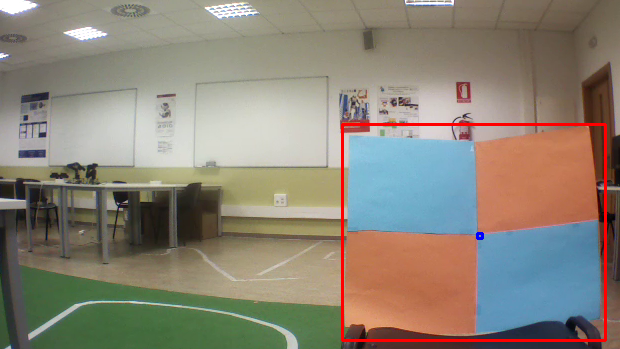
\includegraphics[width=0.29\textwidth]{imgs/k_beacon21.png}}
  \subfloat[Suma de objetos]{
   \label{f:sumaobjetos}
    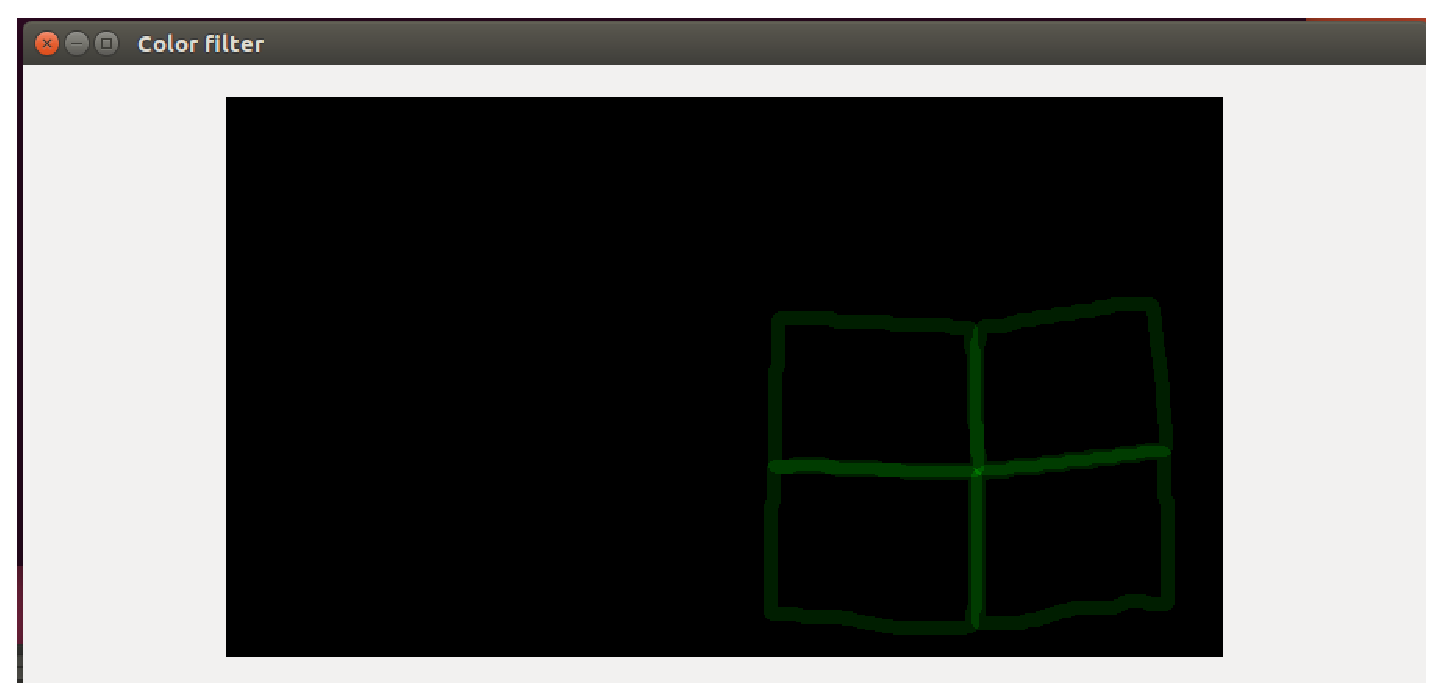
\includegraphics[width=0.33\textwidth]{imgs/k_Beacon1.eps}} 
 \caption{Procesamiento de imagen de la baliza}
 \label{f:ColorFilterTotal}
\end{figure} 



\section{Control}
\label{sec.control}

\hspace{1 cm} En \'esta secci\'on se explica el control sobre el drone en funci\'on del momento en el que se encuentra y la imagen que se obtiene. Se puede dividir \'esta secci\'on en tres partes:
despegue, b\'usqueda y aterrizaje.


\subsection{Despegue}

\hspace{1 cm} Esta fase est\'a controlada por tiempo. Son los primeros diez segundos del algoritmo, y en ellos el drone despega de forma controlada. Esta fase ser\'a "`Take off"' en el aut\'omata de estados.  Para ello se sit\'ua el drone sobre una baliza sobre la cual tiene que estabilizarse. De esta forma, al despegar detecta \'esta y trata de centrarse, evitando as\'i que se desv\'ie por factores externos y qued\'andose en la situaci\'on correcta. Debido a que el drone va a despegar sobre la baliza, el control en esta parte es un control proporcional, para evitar que tenga que hacer m\'ultiples operaciones, por tanto sea mas r\'apido el algoritmo, y suficiente para ser controlado.



\subsection{B\'usqueda}
\hspace{1 cm} Esta fase comenzar\'a cuando finalicen los diez segundos de despegue. El drone comenzar\'a a navegar de forma aut\'onoma en busqueda de una baliza sobre la cual aterrizar. Para ello comenzar\'a un algoritmo en espiral, estado "`Search"', de forma que ira rastreando la zona ampliando su giro de forma continua, hasta que detecte una posible baliza. En el momento que la detecte, pasar\'a al estado "`Possibly beacon"' e intentara centrarse sobre ella. En caso de no tratarse de la baliza continuara con el algoritmo de b\'usqueda, pero en caso de serlo pasar\'a al estado "`Centering beacon"', haciendo que coincida el centro de la baliza con el centro de la imagen de la c\'amara. Para realizar el movimiento de centrarse en la baliza se ha utilizado un control PID(progresivo, integral y derivativo). Esto se debe a que solo con el control progresivo, se produc\'ia una gran diferencia de velocidad y el drone cambiaba sus giros de forma muy brusca, lo que le llevaba a desestabilizarse y perder con facilidad la baliza.  Este control se basa en derivar el error con respecto al tiempo y multiplicarlo por una constante. Dado que nuestro algoritmo ejecuta una vez cada cierto tiempo y no esta continuamente pasando por este punto, podemos considerar que se trata de un sistema en tiempo discreto, y por tanto en lugar de trabajar con derivadas trabajaremos con sumatorios. De esta forma, para añadir un control derivativo se realiza una operaci\'on que depende de la velocidad anterior y la que tenemos ahora: \[v_{derivativa} =1-(v_{anterior}-v_{nueva})/50 \] 

\hspace{1cm}Para evitar que el valor sea 0 y al multiplicarlo por el valor progresivo se quede en el sitio, en caso de ser un valor menor a 0.1 se iguala a este. Este resultado lo multiplicamos a la velocidad final, y lo que conseguimos es que si el valor entre dos velocidades continuas es muy alto este se aten\'ue de forma que el drone no cambie mucho y vaya oscilando, sino que lleve una velocidad mas continua a la hora de acelerar o frenar.  

El siguiente fragmento de c\'odigo consigue que el drone se mueva realizando espirales:

\begin{lstlisting}[backgroundcolor=\color{yellow}]
self.cmdvel.sendCMDVel(1.8+wSearch,0,0,0,0,1.5 - wSearch)
numVuelta=numVuelta+1
if(numVuelta==100):
    timerW=timerW+(timerW/8)
    numVuelta=0
    if(wSearch<1):
        wSearch=wSearch+0.2
\end{lstlisting}

\hspace{1cm} Para visualizar el diagrama de estados, se tuvieron que añadir dos paquetes del GUI de JdeRobot, uno que permit\'ia abrir otra ventana y otro que permit\'ia añadir estados y transiciones entre ellos. Para marcarlo, siendo el numero que aparece el numero del estado que queremos marcar, val\'ia con la siguiente linea de c\'odigo:

\begin{lstlisting}
self.machine.setStateActive(2, True)
\end{lstlisting}
	
\hspace{1cm}La imagen del diagrama que ver\'iamos durante la ejecuci\'on se encuentra en \ref{fig:Diag_estados}.

\subsection{Aterrizaje}

\hspace{1 cm} Esta fase es un aterrizaje controlado, en el cual, una vez que el drone se ha centrado sobre la baliza comienza a descender, cambiando su estado a "`Landing"', y una vez el area de la baliza es suficiente, como para detectar que el drone est\'a muy pr\'oximo a ella, se env\'ia la instrucci\'on land, aterrizando de \'esta forma el drone, siendo aqu\'i su estado "`Landed"'. El hecho de enviarse la orden de aterrizar cuando se esta a una distancia cercana a la baliza es porque esta instrucci\'on es a ciegas, una vez que se env\'ia el drone solo se encarga de descender hasta que nota que est\'a sobre un lugar sobre el cual posarse. Por lo tanto si se env\'ia esta orden a una distancia lejana, el drone puede perder la referencia y aterrizar en otro sitio. 























